%!TEX root = main.tex

\textbf{Problem 1:} \textit{Bernoulli GLMs as a latent variable models.}

Consider a Bernoulli regression model,
\begin{align*}
    w &\sim \cN(\mu, \Sigma) \\
    y_n \mid x_n, w &\sim \mathrm{Bern}(f(w^\trans x_n)) \quad \text{for } n = 1,\ldots, N,
\end{align*}
where $w$ and $x_n$ are vectors in $\reals^D$, $y_n \in \{0, 1\}$, and $f: \reals \to [0, 1]$ is the mean function. In class we studied Newton's method for finding the maximum a posteriori (MAP) estimate~$w^\star = \argmax p(w \mid \{x_n, y_n\}_{n=1}^N)$.  Now we will consider methods for approximating the full posterior distribution.

\begin{enumerate}[label=(\alph*)]
% ======================================================
\item Rather than using the logistic function, let the mean function be the normal cumulative distribution function (CDF), or ``probit'' function,
\begin{align*}
    f(u) &= \Pr(z \leq u) \text{ where } z \sim \cN(0, 1) \\
    &= \textstyle\int_{-\infty}^u \cN(z; 0, 1) \, \mathrm{d}z.
\end{align*}
This is called the probit regression model.  Show that the likelihood~$p(y_n \mid x_n, w)$ is a marginal of a joint distribution,
\begin{align*}
    p(y_n, z_n \mid x_n, w) &= \bbI[z_n \geq 0]^{\bbI[y_n = 1]} \, \bbI[z_n < 0]^{\bbI[y_n = 0]} \cN(z_n \mid x_n^\trans w, 1).
\end{align*}


\begin{solution}
% ------------------------------------------------------------------
The product of expressions raised to an indicator function can be equivalently written as the sum of the expressions times the indicator function. For the augmented joint distribution, we have
\begin{align*}
    p(y_n, z_n \mid x_n, w)
        &=  \bbI[z_n \geq 0]^{\bbI[y_n = 1]} \,
            \bbI[z_n < 0]^{\bbI[y_n = 0]}
            \cN(z_n \mid x_n^\trans w, 1)\\
        &=  \bbI[y_n = 1]\,\bbI[z_n \geq 0] \,
            \cN(z_n \mid x_n^\trans w, 1)
            + \bbI[y_n = 0]\,\bbI[z_n < 0] \,
            \cN(z_n \mid x_n^\trans w, 1)
\end{align*}
Now, when we integrate over $z_n$ to recover the marginal disribution of $y_n$, we can split the integral into a sum of two disjoint integration limits:
\begin{align*}
    p(y_n \given x_n, w)
        &= \textstyle\int_{-\infty}^\infty p(y_n, z_n \given x_n, w) \\
        &= \textstyle\int_{-\infty}^0
                \bbI[y_n = 1]\,
                \cN(z_n \mid x_n^\trans w, 1) \mathrm{d}z_n
            + \textstyle\int_{0}^\infty
                \bbI[y_n = 0]
                \cN(z_n \mid x_n^\trans w, 1) \mathrm{d}z_n\\
        &= \bbI[y_n = 1]\,
                \textstyle\int_{-\infty}^{x_n^\trans w}
                \cN(z_n \mid 0, 1) \mathrm{d}z_n
            + \bbI[y_n = 0]
                \textstyle\int_{x_n^\trans w}^\infty
                \cN(z_n \mid 0, 1) \mathrm{d}z_n\\
        &= \bbI[y_n = 1]\, f(x_n^\trans w)
            + \bbI[y_n = 0]\,(1-f(x_n^\trans w)) \\
        &= \distBernoulli(y_n \given x_n^\trans w)
\end{align*}

% ------------------------------------------------------------------
\end{solution}


% ======================================================
\clearpage
\item Derive the conditional distributions~$p(w \mid \{x_n, y_n, z_n\}_{n=1}^N)$ and~$p(z_n \mid x_n, y_n, w)$.\footnote{Observe that $z_n$ is conditionally independent of $\{x_{n'}, y_{n'}, z_{n'}\}_{n' \neq n}$ given $w$.}

\begin{solution}
%------------------------------------------------------------------
Posterior on $w$:
\begin{align*}
    p(w \mid \{x_n, y_n, z_n\}_{n=1}^N)
        &\propto \prod_n p(y_n, z_n, w \given x_n) \\
        &\propto p(w) \prod_n p(y_n, z_n \given x_n, w) \\
        &\propto \cN(\mu, \Sigma)
            \prod_n
                \bbI[z_n \geq 0]^{\bbI[y_n = 1]} \,
                \bbI[z_n < 0]^{\bbI[y_n = 0]}
                \cN(z_n \mid x_n^\trans w, 1) \\
    p(z_n \mid x_n, y_n, w) 
        &\propto p(y_n, z_n \given x_n, w) \\
        &\propto \bbI[z_n \geq 0]^{\bbI[y_n = 1]} \,
                \bbI[z_n < 0]^{\bbI[y_n = 0]}
                \cN(z_n \mid x_n^\trans w, 1) \\
        &\propto \bbI[y_n = 1]\,\bbI[z_n \geq 0] \,
            \cN(z_n \mid x_n^\trans w, 1)
            + \bbI[y_n = 0]\,\bbI[z_n < 0] \,
            \cN(z_n \mid x_n^\trans w, 1)
\end{align*}

%------------------------------------------------------------------
\end{solution}

\item \emph{Gibbs sampling} is a Markov chain Monte Carlo (MCMC) method for approximate posterior inference.  It works by repeatedly sampling from the conditional distribution of one variable, holding all others fixed.  For the probit regression model, this means iteratively performing these two steps:
\begin{enumerate}[label=\arabic*.]
    \item Sample $z_n \sim p(z_n \mid x_n, y_n, w)$ for~$n = 1, \ldots, N$ holding ~$w$ fixed;
    \item Sample $w \sim p(w \mid \{x_n, y_n, z_n\}_{n=1}^N)$ holding $\{z_n\}_{n=1}^N$ fixed.
\end{enumerate}
Note the similarity to EM: rather than computing a posterior distribution over~$z_n$, we draw a sample from it; rather than setting~$w$ to maximize the ELBO, we draw a sample from its conditional distribution.  It can be shown that this algorithm defines a Markov chain on the space of $(w, \{z_n\}_{n=1}^N)$ whose stationary distribution is the posterior~$p(w, \{z_n\}_{n=1}^N \mid \{x_n, y_n\}_{n=1}^N)$.  In other words, repeating these steps infinitely many times would yield samples of~$w$ and~$\{z_n\}_{n=1}^N$ drawn from their posterior distribution. 

Implement this Gibbs sampling algorithm and test it on a synthetic dataset with~$D=2$ dimensional covariates and~$N=100$ data points.  Scatter plot your samples of~$w$ and, for comparison, plot the true value of~$w$ that generated the data. Do your samples look approximately Gaussian distributed?  How does the posterior distribution change when you vary~$N$? 

\begin{solution}
This figure was generated together with Tucker and Minseung.
\begin{figure}[htb]
    \centering
    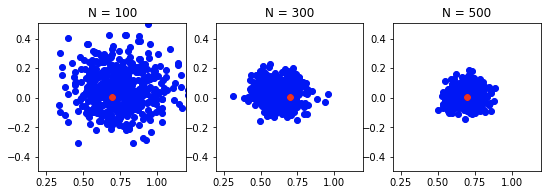
\includegraphics[width=0.5\textwidth]{1c_image.png}
    \caption{Samples of $w$ for different size datasets, vs. true value of $w$ (red). As we increase $N$, the posterior distribution has increasingly smaller variance, which is consistent with having more observations.}
\end{figure}
\end{solution}

\item \textbf{Bonus.}  There are also auxiliary variable methods for logistic regression, where~$f(u) = e^u / (1+e^u)$.  Specifically,  we have that,
\begin{align*}
    \frac{e^{y_n \cdot w^\trans x_n}}{1 + e^{w^\trans x_n}} &= 
    \int_0^\infty \tfrac{1}{2} \exp \left\{ \big(y_n - \tfrac{1}{2}\big) x_n^\trans w -\tfrac{1}{2} z_n (w^\trans x_n)^2 \right\} \mathrm{PG}(z_n; 1, 0) \, \mathrm{d}z_n,
\end{align*}
where~$\mathrm{PG}(z; b, c)$ is the density function of the \emph{P\'{o}lya-gamma} (PG) distribution over~$z \in \reals_+$ with parameters~$b$ and $c$.   The PG distribution has a number of nice properties: it is closed under exponential tilting so that,
\begin{align*}
    e^{-\tfrac{1}{2} z c^2} \, \mathrm{PG}(z; b, 0) \propto \mathrm{PG}(z; b, c),
\end{align*}
and its expectation is available in closed form,
\begin{align*}
    \bbE_{z \sim \mathrm{PG}(b, c)}[z] &= \frac{b}{2c} \tanh \left(\frac{c}{2} \right).
\end{align*}
Use these properties to derive an EM algorithm for finding~$w^\star = \argmax p(\{y_n\} \mid \{x_n\}, w)$.  How do the EM updates compare to Newton's method?

\end{enumerate}
